\chapter{Zadanie 2}
	\label{ch:zadanie2}
	
	\section{Obiekt rozmyty}
		\label{sec:ob_roz}
		Utworzenie modelu rozmytego Takagi-Sugeno dla obiektu należy zacząć od wyznaczenia funkcji przynależności. Jako funkcji przynależności zdecydowaliśmy się użyć funkcji sigmoidalnych. Ponieważ projekt zakłada utworzenie modeli rozmytych z dwoma, trzema, czterema oraz pięcioma modelami lokalnymi, funkcje przynależności dla pierwszego, n-tego oraz ostatniego (przy r obecnych modelach lokalnych) modelu lokalnego wyglądają tak jak w równaniach od \ref{eq:sig1} do \ref{eq:sigost}. W podanych wzorach zmienna a oznacza nachylenie funkcji i została przyjęta taka sama dla wszystkich modeli lokalnych. Wektor c natomiast zawiera punkty dla których funkcje przynależności sąsiednich modeli lokalnych osiągają wartość 0.5. Wartość a została dobrana eksperymentalnie na poziomie a=3. Wartości c zostały wyliczone poprzez podzielenie zakresu wartości zmiennej na podstawie której liczony jest obiekt rozmyty przez ilość regulatorów lokalnych, co zagwarantowało w równomierny podział zbiorów rozmytych. Zdecydowaliśmy się na wykorzystanie wyjścia obiektu jako zmiennej determinującej zbiory rozmyte. Decyzja ta poparta była faktem, że dla sterowania w obiekcie występuje znaczne opóźnienie co prawdopodobnie uniemożliwiłoby późniejsze zaimplementowanie na utworzonych zbiorach rozmytych skutecznie działającego regulatora. Dla badanego w zadaniu pierwszym zakresu sterowań wyjście obiektu przyjmuje wartości w przybliżeniu od 4.5 do 34.5, dlatego właśnie w takim zakresie tworzone były zbiory rozmyte. Dodatkowo dla każdego zbioru rozmytego należało określić punkt pracy w którym zlinearyzowany był obiekt lokalny. Punkty pracy zostały wyznaczone na podstawie kształtu poszczególnych funkcji przynależności. Wartość wyjścia w punkcie pracy dla wybranego modelu równa jest w przybliżeniu wartości wyjścia znajdującej się w środku przedziału dla którego funkcja przynależności wynosi 1. Funkcje przynależności dla utworzonych obiektów rozmytych przedstawione zostały na wykresach od \ref{rys:roz2} do \ref{rys:roz5}.
		
		\begin{equation}
			\mu(1) = 1-\frac{1}{1+e^{-a*(h2-c(1))}}
			\label{eq:sig1}
		\end{equation}
		\begin{equation}
			\mu(n) = \frac{1}{1+e^{-a*(h2-c(n-1))}}-\frac{1}{1+e^{-a*(h2-c(n))}}
			\label{eq:sign}
		\end{equation}
		\begin{equation}
		\mu(r) = \frac{1}{1+e^{-a*(h2-c(r-1))}}
		\label{eq:sigost}
		\end{equation}
		
		\begin{figure}[h!]
			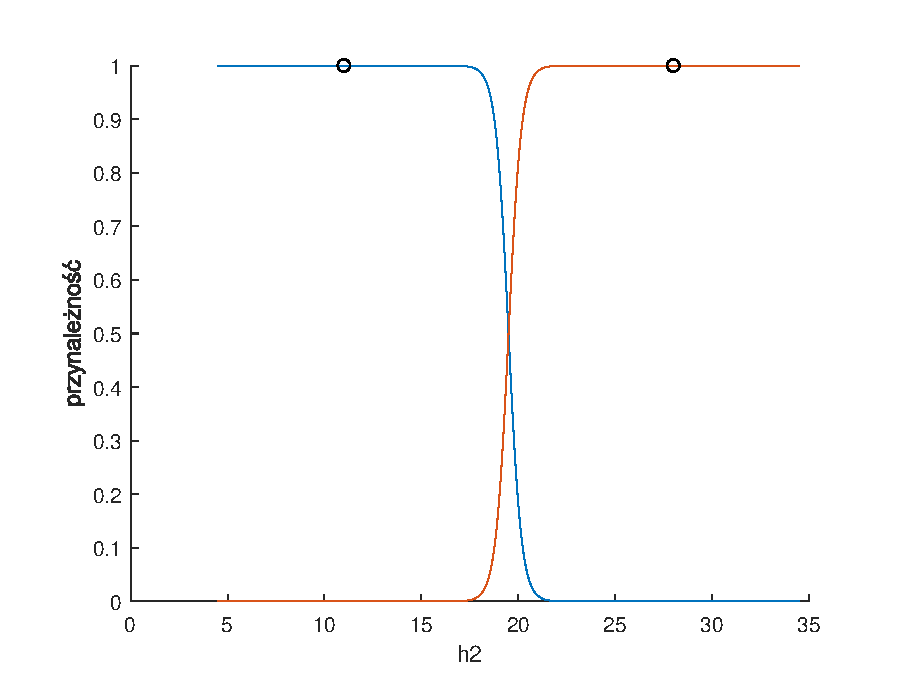
\includegraphics[width=0.9\linewidth]{plots/z2_modelroz_2.eps}
			\caption{Funkcje przynależności dla obiektu rozmytego z dwoma obiektami lokalnymi}
			\label{rys:roz2}
		\end{figure}
		\begin{figure}[h!]
			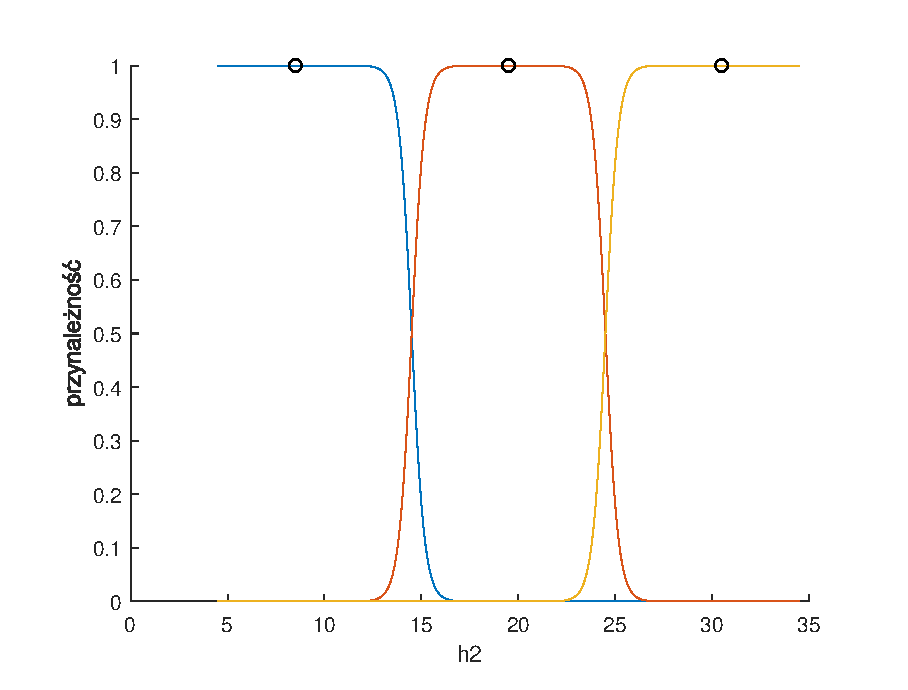
\includegraphics[width=0.9\linewidth]{plots/z2_modelroz_3.eps}
			\caption{Funkcje przynależności dla obiektu rozmytego z trzema obiektami lokalnymi}
			\label{rys:roz3}
		\end{figure}
		\begin{figure}[h!]
			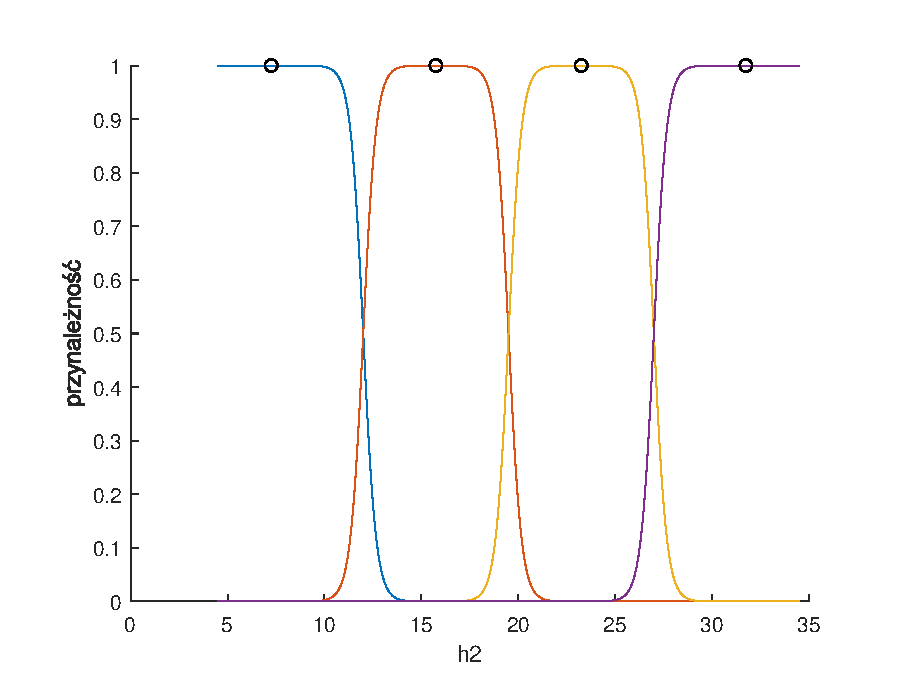
\includegraphics[width=0.9\linewidth]{plots/z2_modelroz_4.eps}
			\caption{Funkcje przynależności dla obiektu rozmytego z czterema obiektami lokalnymi}
			\label{rys:roz4}
		\end{figure}
		\begin{figure}[h!]
			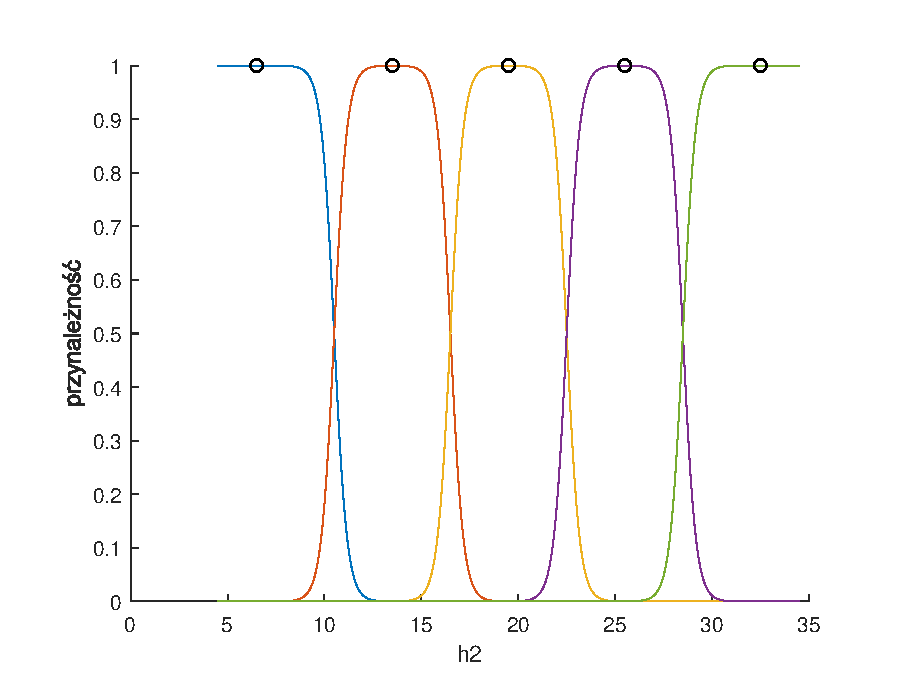
\includegraphics[width=0.9\linewidth]{plots/z2_modelroz_5.eps}
			\caption{Funkcje przynależności dla obiektu rozmytego z pięcioma obiektami lokalnymi}
			\label{rys:roz5}
		\end{figure}
	
	
		Utworzenie obiektu rozmytego na podstawie przedstawionych funkcji przynależności nie sprawiło już zbytniego problemu. Zakładając, że obiekt ma określoną ilość zbiorów rozmytych i każdy zbiór posiada swój punkt linearyzacji zaimplementowane została określona ilość obiektów liniowych. W każdej iteracji liczone są wyjścia wszystkich obiektów liniowych oraz wagi według funkcji przynależności. Następnie faktyczny stan obiektu otrzymywany jest poprzez przemnożenie wyników lokalnych przez ich wagi i podzielenie otrzymanej liczby przez sumę wag. Oczywiście dla każdego modelu liniowego potrzebny jest punkt linearyzacji, który jak już wspominałem został określony jedynie poprzez wartość wyjścia obiektu $h_{20}$. Wartości $V_{10}$, $V_{20}$ oraz $h_{10}$ obliczane są analogicznie jak dla obiektu liniowego z pierwszego zadania. Co do wartości zakłócenia $F_{D0}$ ustalona została ona na 10. Wartość sterowania w punkcie linearyzacji $F_{10}$ można zatem wyliczyć podstawiając wartość 0 pod pochodną $dV/dt$, co daje nam działanie $F_{10} = \alpha_1*\sqrt{h_{20}}-F_{D0}$.
		
		Porównania działania poszczególnych modeli rozmytych modelem nieliniowym oraz liniowym obiektu przedstawione zostały na wykresach od \ref{rys:roz2p} do \ref{rys:roz5p}. Dla każdego modelu wykonane zostały przebiegi ze skokami sterowania w kroku 100. Użyte skoki sterowania są takie same jak w zadaniu pierwszym. Na wykresach przebiegi dla oryginalnego obiektu przedstawione są kolorem niebieskim, dla zlinearyzowanego różowym, a dla rozmytego zielonym.
		
		Dla modelu z dwoma obiektami lokalnymi działanie modelu rozmytego definitywnie nie jest zadowalające. Końcowa wartość wyjścia obiektu rozmytego w większości przypadków zauważalnie rozbiega się z końcową wartością dla oryginalnego modelu. Kształty przebiegów dla poszczególnych skoków nie są podobne do przebiegów nieliniowego ani liniowego obiektu. Przebiegiem, który najbardziej pokrywa się z oryginałem jest ten dla skoku sterowania do 34 (drugi od dołu).
		
		Dla modelu z trzema obiektami lokalnymi sytuacja wydaje się lepsza. Przebiegi dla skoków powyżej punktu pracy są zbliżone w wyglądzie do oryginalnego obiektu. Nie licząc przebiegu dla skoku sterowania do 24 (pierwszy od dołu) wartości końcowe wyjścia obiektu rozmytego w przybliżeniu pokrywają się z wartościami dla obiektu oryginalnego.
		
		Dla modelu z czterema obiektami lokalnymi znowu nastąpiła nieznaczna poprawa. Przebiegi przez większość symulacji pokrywają się kształtem z przebiegami dla pierwotnego modelu, jednakże część wartości końcowych wyjścia nieznacznie odbiega od pożądanych.

		Modelu z pięcioma obiektami lokalnymi działa najlepiej z przedstawionych. Poza kilkoma miejscami przebiegi pokrywają się z przebiegami dla oryginalnego obiektu. Wartości końcowe także są w przybliżeniu równe wartościom końcowym dla obiektu oryginalnego. Obiekt ten jest zdecydowanie najlepszym z utworzonych i to właśnie on wykorzystywany będzie do dalszych badań.
		
		Badanie to ukazuje jak przydatne mogą być modele rozmyte przy modelowaniu obiektów nieliniowych. Działanie modelu liniowego w dużej odległości od punktu pracy zbyt znacząco różniło się od działania modelu nieliniowego, by można było stosować je zamiennie. Dzięki wykorzystaniu kilku modeli liniowych sprzężonych w model rozmyty jesteśmy w stanie dosyć dokładnie odwzorować obiekt, co potencjalnie umożliwiałoby stosowanie modelu rozmytego zamiast oryginału.
		
		Pomimo prób nie udało się znaleźć lepszego modelu rozmytego, czyli takiego, który niwelowałby znacząco wady modelu otrzymanego automatycznie (różnice w przebiegach funkcji dla skoków do niskich sterowań) nie pogarszając działania reszty modelu. Z tego powodu podtrzymaliśmy naszą decyzję o używaniu wygenerowanych dla 5 modeli lokalnych funkcji przynależności.
		
		\begin{figure}[h!]
			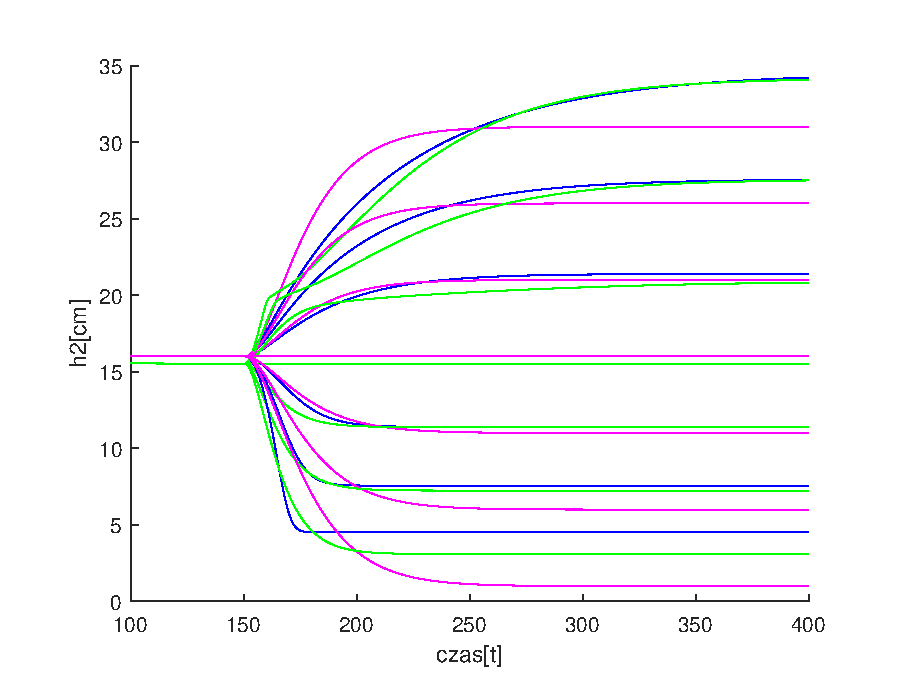
\includegraphics[width=0.9\linewidth]{plots/z2_modelroz_2p.eps}
			\caption{Porównanie działania dla obiektu rozmytego z dwoma obiektami lokalnymi}
			\label{rys:roz2p}
		\end{figure}
		\begin{figure}[h!]
			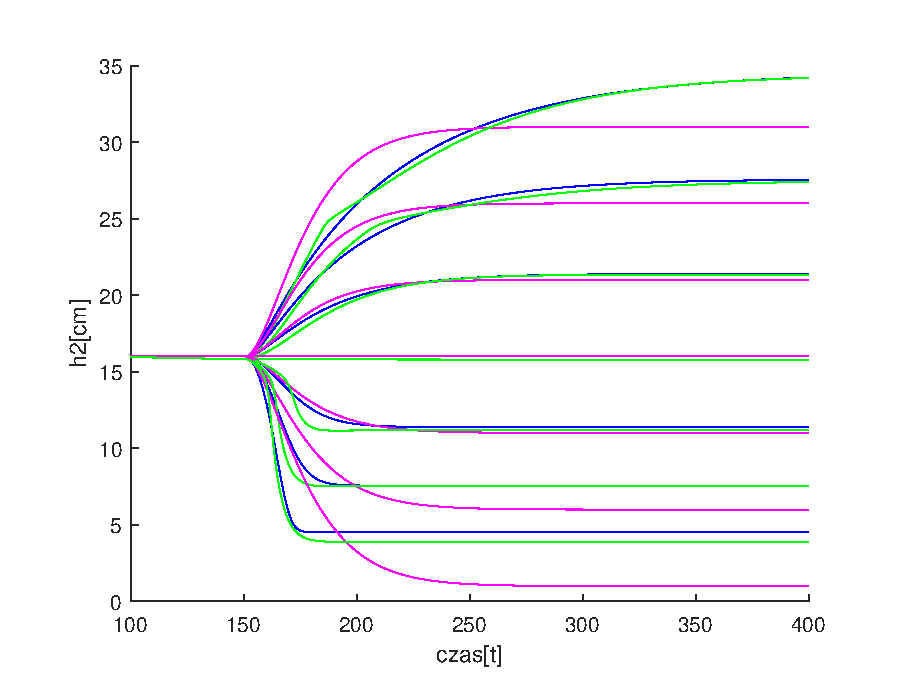
\includegraphics[width=0.9\linewidth]{plots/z2_modelroz_3p.eps}
			\caption{Porównanie działania dla obiektu rozmytego z trzema obiektami lokalnymi}
			\label{rys:roz3p}
		\end{figure}
		\begin{figure}[h!]
			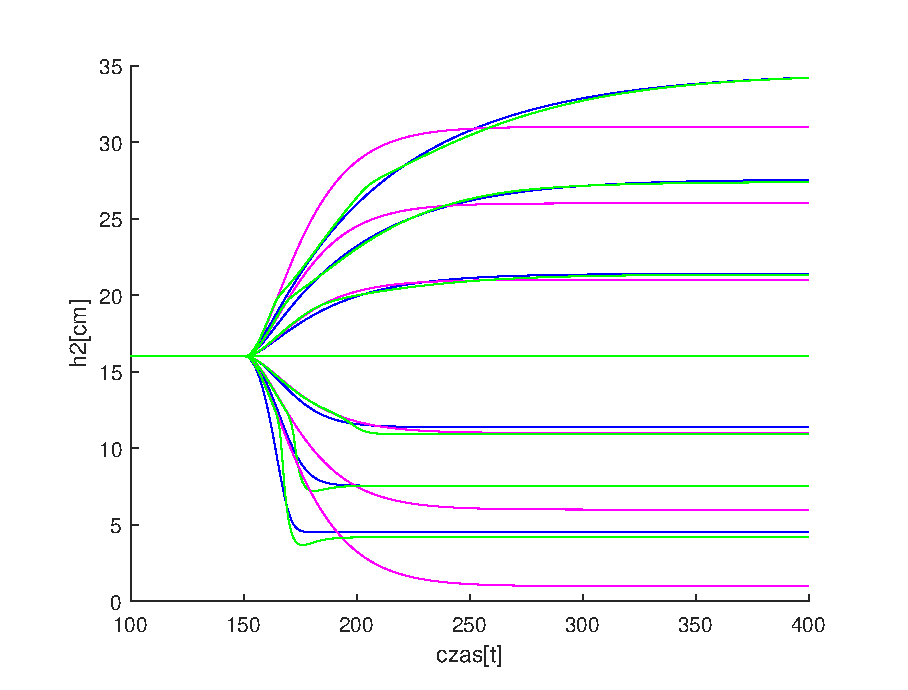
\includegraphics[width=0.9\linewidth]{plots/z2_modelroz_4p.eps}
			\caption{Porównanie działania dla obiektu rozmytego z czterema obiektami lokalnymi}
			\label{rys:roz4p}
		\end{figure}
		\begin{figure}[h!]
			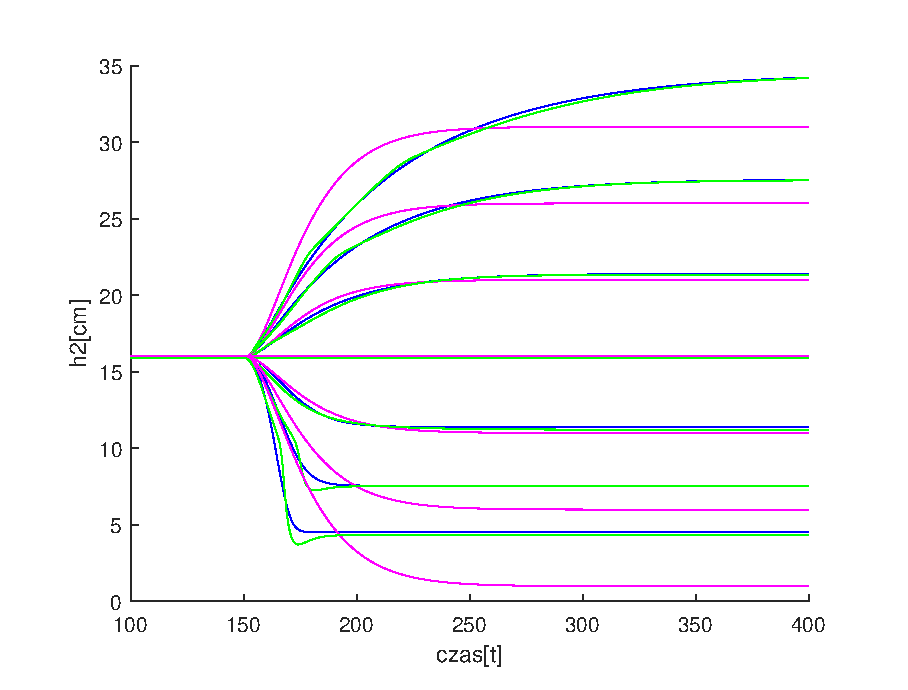
\includegraphics[width=0.9\linewidth]{plots/z2_modelroz_5p.eps}
			\caption{Porównanie działania dla obiektu rozmytego z pięcioma obiektami lokalnymi}
			\label{rys:roz5p}
		\end{figure}
	\newpage
	\section{DMC rozmyty}\
		Implementacja rozmytego regulatora DMC nie jest bardzo skomplikowana. W tym celu należy zaimplementować tyle regulatorów DMC ile jest zbiorów rozmytych, w naszym wypadku 5. Regulatory różnią się między sobą odpowiedziami skokowymi, które są zebrane w punktach pracy odpowiadających każdemu z modelów. W każdym kroku regulacji każdy z regulatorów lokalnych oblicza zmianę sterowania. Następnie obliczane są wagi poszczególnych zbiorów rozmytych i następuje rozmycie zmiany sterowania. Każde z wyliczonych sterowań przemnażane jest przez swoją wagę, wyniki sumuje się i dzieli przez sumę wag otrzymując w ten sposób końcową zmianę sterowania.
		
		Dodatkowo w wymaganiach napisane było, że regulator rozmyty powinien posiadać ograniczenia. W tym celu przyjęte zostały przez nas: maksymalna wartość sterowania - 90, minimalna wartość sterowania - 20 oraz maksymalna zmiana sterowania w jednym kroku - 1. Ograniczenia te uwzględnia się dopiero po obliczeniu końcowej wartości zmiany sterowania.
		
		Stworzony na podstawie wyznaczonych funkcji przynależności regulator rozmyty otrzymał takie same zadanie wyregulowania obiektu jak zwykły regulator w zadaniu pierwszym. Początkowo wartości wszystkich horyzontów zostały ustawione na najwyższą wartość, czyli długość odpowiedzi skokowej - 400, a lambda na wartość dla której przebieg zwykłego regulatora wydał nam się optymalny - 2000. Przebiegi regulacji obiektu dla tych parametrów zostały przedstawione na wykresie \ref{rys:dmcoryg}. Jak widać przebiegi są bardzo dobre, a w porównaniu z przebiegami pojedynczego DMC dla tej samej lambdy wręcz genialne. Błąd regulacji także jest mniejszy i wynosi 18.2898. Obiekt dąży do zadanej wartości wyjścia bez oscylacji ani przesterowań i osiąga go dość szybko.
		
		Po tak spektakularnym sukcesie oryginalnego kształtu funkcji rozpoczęliśmy eksperymenty nad jego zmianą w celu dalszej optymalizacji regulacji. Po wielu próbach przystaliśmy na kształt przedstawiony na rysunku \ref{rys:dmcprzyn}. Przebieg regulacji dla tak skonstruowanych zbiorów rozmytych przedstawiony jest na wykresie \ref{rys:dmcroz2000}. Jak widać nie uległ on znaczącej zmianie. Błąd regulacji dla zmienionej funkcji przynależności wyniósł jednak nieco mniej, a dokładnie 18.2504.
		
		Po zmianie właściwości rozmycia zdecydowaliśmy się jeszcze sprawdzić działanie dla mniejszych wartości lambda, a dokładnie dla lambda równego 100, dla którego oryginalny DMC nie radził sobie dobrze z regulacją, powodując gasnące oscylacje dla wysokich skoków wartości zadanej. Przebieg dla zmniejszonej lambdy przedstawiony został na wykresie \ref{rys:dmcroz100}. Jak widać uległ on nieco pogorszeniu, zaczęły występować niewielkie przesterowania oraz pojedyncze oscylacje. Z drugiej strony błąd sterowania zmalał prawie o jedną trzecią swojej dotychczasowej wartości, aż do 13.6096. Zdecydowaliśmy, że niewielkie pogorszenie przebiegów jest małą ceną za znacznie niższy błąd i pozostaliśmy przy zmienionej wartości lambda.
		
		Ostatnią rzeczą jaką regulowaliśmy dla zaimplementowanego regulatora rozmytego jest zmiana długości horyzontów. Zdecydowaliśmy się na ten krok, choć zazwyczaj nie przynosi on poprawy regulacji, po części ze względu na kolejne zadania projektu, w których wymagane jest używanie algorytmów optymalizacji, znacznie spowalnianych przez dużą złożoność obliczeniową. Horyzonty skracane były przez nas do momentu, gdy błąd regulacji nie ulegał pogorszeniu. W ten sposób doszliśmy do następujących wartości horyzontów: D = 200, N = 150, Nu = 100, Dz = 200. Przebieg regulacji dla zmniejszonych horyzontów znajduje się na wykresie \ref{rys:dmcroz100hor}. Jak widać nie ma w nim widocznych zmian. Co ciekawe błąd regulacji dla skróconych horyzontów uległ nieznacznej poprawie, do poziomu 13.5395. Nie widząc żadnych przeciwwskazań zdecydowaliśmy o dalszym używaniu skróconych horyzontów w kolejnych zadaniach.
		
		W wykonanych w tym zadaniu przebiegach regulacji można zauważyć działanie ograniczenia wartości sterowania. Jeśli dokładnie przyjrzeć się wykresom zauważalne jest, że ustabilizowana wartość wyjścia obiektu dla czasu w okolicy 4000s jest nieznacznie większa od zadanej. Dzieje się tak, ponieważ sterowanie osiąga swoją wartość minimalną, co spowodowane jest równoczesną obecnością dużego zakłócenia. Przy wystąpieniu spadku zakłócenia w chwili 4600, regulatorowi po chwili udaje się bez problemu osiągnąć zadaną wartość. Ponieważ zachowanie to umożliwia zaobserwowanie zaimplementowanego ograniczenia nie zostało ono usunięte w kolejnych zadaniach, co mogłoby być wykonane dzięki nieznacznemu zwiększeniu dolnej granicy sterowania.
		
		\begin{figure}[h!]
			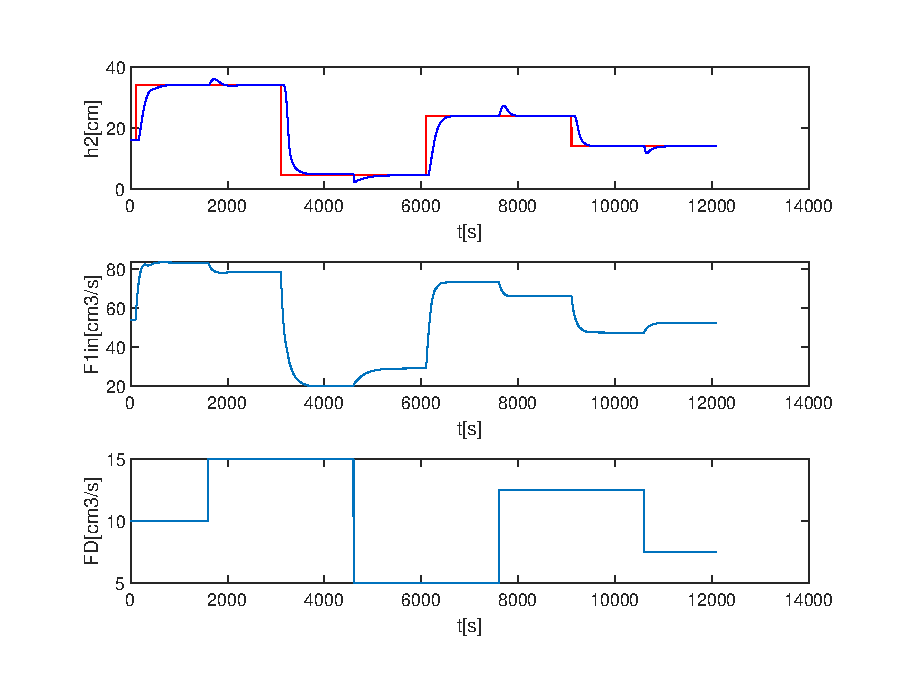
\includegraphics[width=0.9\linewidth]{plots/z2_dmc2000oryg.eps}
			\caption{Przebieg regulacji dla DMC rozmytego przy lambda 2000}
			\label{rys:dmcoryg}
		\end{figure}
		\begin{figure}[h!]
			\includegraphics[width=0.85\linewidth]{plots/z2_dmcprzyn.eps}
			\caption{Zmodyfikowane funkcje przynależności}
			\label{rys:dmcprzyn}
		\end{figure}
		\begin{figure}[h!]
			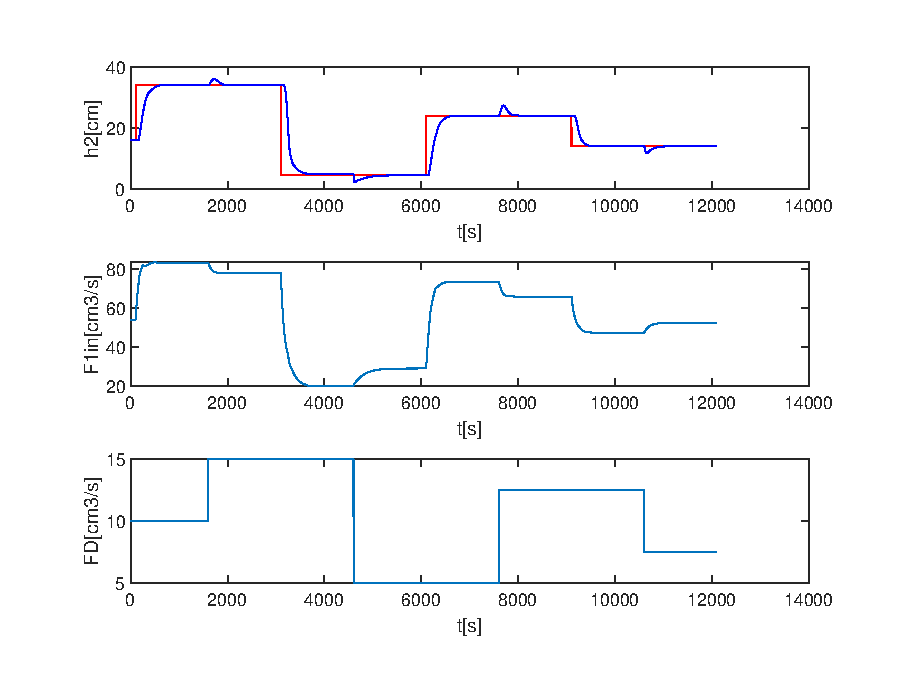
\includegraphics[width=0.9\linewidth]{plots/z2_dmc2000.eps}
			\caption{Przebieg regulacji dla DMC rozmytego przy lambda 2000 i zmodyfikowanych funkcjach przynależności}
			\label{rys:dmcroz2000}
		\end{figure}
		\begin{figure}[h!]
			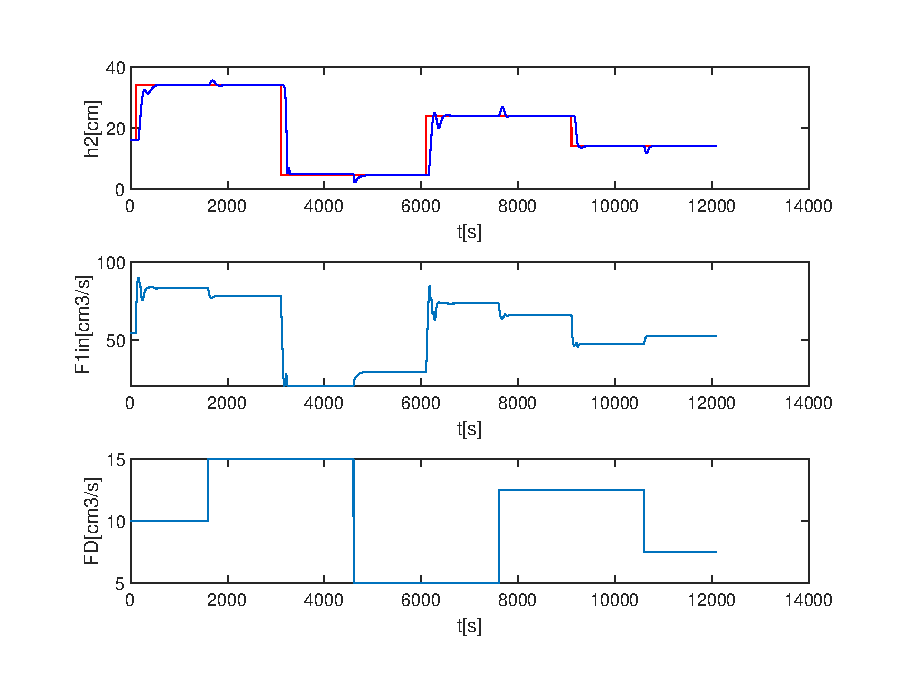
\includegraphics[width=0.9\linewidth]{plots/z2_dmc100.eps}
			\caption{Przebieg regulacji dla DMC rozmytego przy lambda 100}
			\label{rys:dmcroz100}
		\end{figure}
		\begin{figure}[h!]
			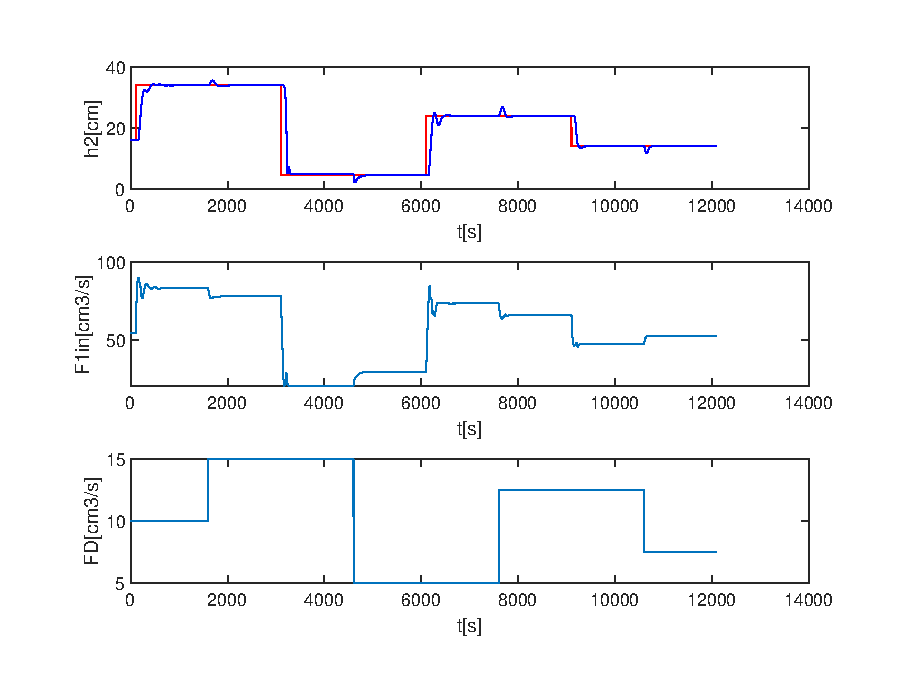
\includegraphics[width=0.9\linewidth]{plots/z2_dmchor.eps}
			\caption{Przebieg regulacji dla DMC rozmytego przy lambda 100 i skróconych horyzontach}
			\label{rys:dmcroz100hor}
		\end{figure}
		